\documentclass[border=0pt]{standalone}
\usepackage[T1]{fontenc}
\usepackage{txfonts}
\usepackage{xcolor}
\usepackage{tikz}
\usetikzlibrary{arrows.meta}

\definecolor{navy}{RGB}{35,74,111}
\definecolor{blue}{RGB}{47,112,164}
\definecolor{teal}{RGB}{45,130,125}
\definecolor{amber}{RGB}{190,119,39}
\definecolor{pale}{RGB}{244,247,250}
\definecolor{ink}{RGB}{37,47,57}
\definecolor{muted}{RGB}{88,101,114}

\begin{document}
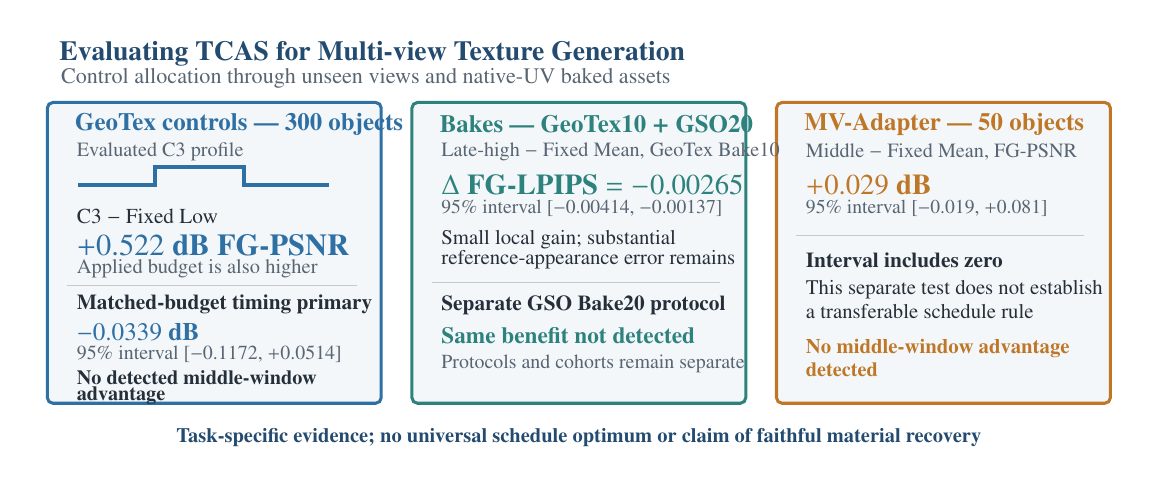
\begin{tikzpicture}[x=1cm,y=1cm]
  % Match the compact landscape footprint of the first-round graphical abstract.
  \useasboundingbox (0,0) rectangle (14,5.55);

  \node[anchor=west,text=navy,font=\bfseries\fontsize{10}{11}\selectfont]
    at (0.28,5.22) {Evaluating TCAS for Multi-view Texture Generation};
  \node[anchor=west,text=muted,font=\fontsize{8}{9}\selectfont]
    at (0.30,4.91) {Control allocation through unseen views and native-UV baked assets};

  % Three evidence panels keep the protocol boundaries visible.
  \foreach \x/\c in {0.25/blue,4.88/teal,9.51/amber} {
    \path[fill=pale,rounded corners=2pt] (\x,0.78) rectangle +(4.24,3.82);
    \draw[\c,line width=1.1pt,rounded corners=2pt] (\x,0.78) rectangle +(4.24,3.82);
  }

  % Fresh C controlled comparison.
  \node[anchor=west,text=blue,font=\bfseries\fontsize{9}{10}\selectfont]
    at (0.48,4.32) {GeoTex controls | 300 objects};
  \node[anchor=west,text=muted,font=\fontsize{7.3}{8}\selectfont]
    at (0.50,3.97) {Evaluated C3 profile};
  \draw[blue,line width=1.4pt] (0.64,3.55)--(1.62,3.55)--(1.62,3.78)--(2.75,3.78)--(2.75,3.55)--(3.83,3.55);
  \node[anchor=west,text=ink,font=\fontsize{7.7}{8.5}\selectfont]
    at (0.50,3.15) {C3 $-$ Fixed Low};
  \node[anchor=west,text=blue,font=\bfseries\fontsize{11}{12}\selectfont]
    at (0.50,2.78) {$+0.522$ dB FG-PSNR};
  \node[anchor=west,text=muted,font=\fontsize{7.4}{8.2}\selectfont]
    at (0.50,2.49) {Applied budget is also higher};
  \draw[muted!35] (0.50,2.28)--(4.18,2.28);
  \node[anchor=west,text=ink,font=\bfseries\fontsize{7.7}{8.5}\selectfont]
    at (0.50,2.03) {Matched-budget timing primary};
  \node[anchor=west,text=blue,font=\bfseries\fontsize{9.1}{10}\selectfont]
    at (0.50,1.68) {$-0.0339$ dB};
  \node[anchor=west,text=muted,font=\fontsize{7.2}{8}\selectfont]
    at (0.50,1.40) {95\% interval [$-0.1172$, $+0.0514$]};
  \node[anchor=west,text=ink,font=\bfseries\fontsize{7.3}{8}\selectfont]
    at (0.50,1.10) {No detected middle-window};
  \node[anchor=west,text=ink,font=\bfseries\fontsize{7.3}{8}\selectfont]
    at (0.50,0.88) {advantage};

  % Native UV bake outcomes.
  \node[anchor=west,text=teal,font=\bfseries\fontsize{9}{10}\selectfont]
    at (5.11,4.32) {Bakes | GeoTex10 + GSO20};
  \node[anchor=west,text=muted,font=\fontsize{7.3}{8}\selectfont]
    at (5.13,3.97) {Late-high $-$ Fixed Mean, GeoTex Bake10};
  \node[anchor=west,text=teal,font=\bfseries\fontsize{10.4}{11}\selectfont]
    at (5.13,3.55) {$\Delta$ FG-LPIPS $=-0.00265$};
  \node[anchor=west,text=muted,font=\fontsize{7.1}{7.8}\selectfont]
    at (5.13,3.25) {95\% interval [$-0.00414$, $-0.00137$]};
  \node[anchor=west,text=ink,font=\fontsize{7.5}{8.3}\selectfont]
    at (5.13,2.86) {Small local gain; substantial};
  \node[anchor=west,text=ink,font=\fontsize{7.5}{8.3}\selectfont]
    at (5.13,2.60) {reference-appearance error remains};
  \draw[muted!35] (5.13,2.31)--(8.79,2.31);
  \node[anchor=west,text=ink,font=\bfseries\fontsize{7.7}{8.5}\selectfont]
    at (5.13,2.02) {Separate GSO Bake20 protocol};
  \node[anchor=west,text=teal,font=\bfseries\fontsize{8.4}{9.1}\selectfont]
    at (5.13,1.64) {Same benefit not detected};
  \node[anchor=west,text=muted,font=\fontsize{7.2}{8}\selectfont]
    at (5.13,1.28) {Protocols and cohorts remain separate};

  % Native MV-Adapter interface outcome.
  \node[anchor=west,text=amber,font=\bfseries\fontsize{9}{10}\selectfont]
    at (9.74,4.32) {MV-Adapter | 50 objects};
  \node[anchor=west,text=muted,font=\fontsize{7.3}{8}\selectfont]
    at (9.76,3.97) {Middle $-$ Fixed Mean, FG-PSNR};
  \node[anchor=west,text=amber,font=\bfseries\fontsize{10.4}{11}\selectfont]
    at (9.76,3.55) {$+0.029$ dB};
  \node[anchor=west,text=muted,font=\fontsize{7.1}{7.8}\selectfont]
    at (9.76,3.25) {95\% interval [$-0.019$, $+0.081$]};
  \draw[muted!35] (9.76,2.91)--(13.42,2.91);
  \node[anchor=west,text=ink,font=\bfseries\fontsize{7.7}{8.5}\selectfont]
    at (9.76,2.60) {Interval includes zero};
  \node[anchor=west,text=ink,font=\fontsize{7.5}{8.3}\selectfont]
    at (9.76,2.22) {This separate test does not establish};
  \node[anchor=west,text=ink,font=\fontsize{7.5}{8.3}\selectfont]
    at (9.76,1.95) {a transferable schedule rule};
  \node[anchor=west,text=amber,font=\bfseries\fontsize{7.5}{8.2}\selectfont]
    at (9.76,1.48) {No middle-window advantage};
  \node[anchor=west,text=amber,font=\bfseries\fontsize{7.3}{8}\selectfont]
    at (9.76,1.20) {detected};

  \node[anchor=center,text=navy,font=\bfseries\fontsize{7.4}{8.2}\selectfont,align=center]
    at (7,0.34) {Task-specific evidence; no universal schedule optimum or claim of faithful material recovery};
\end{tikzpicture}
\end{document}
